\subsubsection{Задача 1.}

Проверить, что векторы следующих систем попарно ортогональны, и дополнить их до ортогональых базисов. $a = \begin{pmatrix}
    1 \\
    -2 \\
    2 \\
    -3
\end{pmatrix}, b =\begin{pmatrix}
    2 \\
    -3\\
    2 \\
    4
\end{pmatrix}$. 

\textbf{Решение.}

Так как у нас базовое обычно скалярное произведение, то проверить, что $(a,b) = 0$ тривиально. Проверив, мы получим, что это и правда так.

Давайте дополним до ортогональных базисов. Сперва дополним до базиса и получим:
$$a = \begin{pmatrix}
    1 \\
    -2 \\
    2 \\
    -3
\end{pmatrix}, b =\begin{pmatrix}
    2 \\
    -3\\
    2 \\
    4
\end{pmatrix}, a_3 = \begin{pmatrix}
    1 \\
    0\\
    0 \\
    0\end{pmatrix}, a_4 = \begin{pmatrix}
    0 \\
    1\\
    0 \\
    0\end{pmatrix} $$
Теперь воспользуемся Грама-Шмидтом и получим ответ.

\subsubsection{Задача 2.}

Найти базис ортогонального дополнения $L^*$ подпространства $L$, натянутого на векторы $a_1 = \begin{pmatrix}
    1 \\
    0\\
    2\\
    1
\end{pmatrix}, a_2 = \begin{pmatrix}
    2 \\
    1 \\ 
    2 \\
    3 
\end{pmatrix}, a_3 = \begin{pmatrix}
    0 \\
    1 \\
    -2\\
    1 \\
\end{pmatrix}$

\textbf{Решение:}

Заметим, что ранг этой системы векторов 2, поэтому выделю базис $a_1,a_3$.

$L^\perp = \begin{cases}
    x_1 + 2x_3 +x_4 = 0\\
    x_2 - 2x_3 + x_4 = 0
\end{cases}$, то есть множество $X$ - множество которое будет выдавать 0 при обычном скалярном произведении с нашими векторами. Решим СЛОУ мы получим базис

\subsubsection{Задача 3.}

Найти ортогональную проекцию $y$ и ортогональную составляющую $z$ вектора $x$. $x = \begin{pmatrix}
    4 \\
    -1 \\
    -3 \\
    4
\end{pmatrix}, L$ натянуто на $a_1 = \begin{pmatrix}
    1 \\
    1\\1\\1
\end{pmatrix}, a_2 =  \begin{pmatrix}
    1 \\
    2 \\
    2 \\
    -1
\end{pmatrix}, a_3 = \begin{pmatrix}
    1 \\
    0\\
    0\\
    3
\end{pmatrix}$

\textbf{Решение:}

Ранг этой системы векторов 2. Возьму 1 и 3 вектор в качестве базиса. $R^4 = L \oplus L^\perp: \forall x \in R^4: x  =y +z$

Заметим, что $y \in L : y = c_1a_1 + c_2a_3$. Поэтому должно быть выполнено:
$$\begin{cases}
    (x,a_1) = c_1(a_1,a_1) + c_2(a_3,a_1)  + (z,a_1)\\
    (x,a_3) = c_1(a_1,a_3)  +c_2(a_3,a_3) + (z,a_3)
\end{cases}$$
Заметим, что $L \perp z$, откуда скалярное равно нуля. Решаю простую СЛНУ для $c_1,c_2$ найдем $y$ и победили.

\subsubsection{Задача 4.}

\begin{center}
   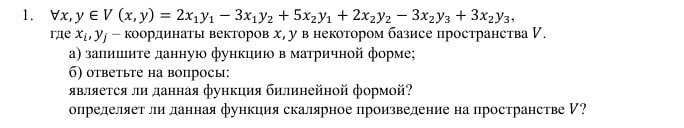
\includegraphics{assets/practice-4-task-4.jpg}
\end{center}

\textbf{Решение:}

Это не билинейная функция и не скалярное (так как на диагонали есть нули)

\subsubsection{Задача 5.}

\begin{center}
   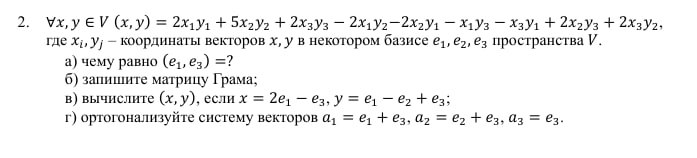
\includegraphics{assets/practice-4-task-5.jpg}
\end{center}

\textbf{Решение:}

$(e_1,e_3 ) = -1$. $G = \begin{pmatrix}
    2 & -2 & -1\\
    -2 &5 & 2 \\
    -1 & 2 &2
\end{pmatrix}$

Заметим, что на диагонали числа больше 0, а также симметричная форма.
$$(x,y) = x^T G y = \begin{pmatrix}
    2 & 0 & 1 
\end{pmatrix} G \begin{pmatrix}
    1 \\
    -1\\
    1
\end{pmatrix} = 7$$

Чтобы ортогонализовать систему векторов надо не забыть, что у нас новое скалярное произведение, которое задается через матрицу Грама. А так обычный ГМШ.